\chapter{Networks}

Computing devices have been in use for thousands of years, at least since the invention of the Sumerican abacus between four and five thousand years ago. Even as computers became more sophisticated, a long process culminating in the development of transistor-based digital computers, they remained specialized machines, largely for use in government or business settings. The explosion in personal computing, which has flooded the planet with billions of computers that pervade almost every aspect of society, coincided roughly with the development of computer networking and the Internet. Communicating via computers -- with friends, news outlets, vendors, banks, or even artificial intelligence systems -- has revolutionized the way the world works.

In this chapter, we'll learn how computer networks work, from the wires in the ground up to the more familiar technologies in a browser or email client. The Internet is one of the largest and most complex machines ever built, so we certainly won't be able to cover every aspect of it, but we'll focus on a few important topics. After reading, you should be able to tell a story about what happens when you open a website or send an email, and understand how to get under the hood and see how different pieces are working together to complete the task.

In addition to its inherent interest, understanding networks is very practical. Many companies look for Internet Technology or IT specialists who understand how networks work. Taking a test like the Network+ certification or A+ certification allows access to these jobs. These tests are knowledge based, so you don’t need practical experience to do well on them. They qualify you for entry level positions that pay around \$50,000 a year. If you're interested in preparing for these exams, there are many books that can help you prepare. For instance, ``CompTIA A+ Certification All-in-One Exam Guide, Ninth Edition (Exams 220-901 \& 220-902).''

\section{Network Layers}\label{sec:network:layers}

Before the Internet, the most popular method of communication at a distance was the postal system. In many ways, the Internet is a much faster and more automated version of the postal system. In particular, the Internet is built up from several different layers. Let's consider the following example of a letter being sent from Alice at Acme, Inc. to Bob at Boxes, Inc.:

\begin{enumerate}
    \item Alice tells her employee, Jane, to order 50 new boxes. Jane drafts a letter to Bob at Boxes, Inc.: ``Please send 50 boxes.'' She seals it in an envelope, opens her address book and copies down Bob's mailing address, and drops the envelope off at the company mailroom. A worker in the mailroom sees that the letter is addressed to a destination outside Acme, Inc., and so he places the envelope in a postal box outside.
    \item A postal worker picks up the envelop from the postal box, and sees that the letter is addressed to a location outside the city. He brings the letter to the local post office, and places it into a bin to be sorted.
    \item Another postal worker picks up the envelope from the bin, and puts it on a mail truck destined for Bob's city.
    \item The mail truck drives along a highway from Alice's city to Bob's city, and gives the letter to the post office there.
    \item A postal worker in Bob's city carries the envelope to Boxes, Inc., and places it in their mailbox.
    \item A worker in the mailroom sees the envelope addressed to Bob. She brings it to Bob's office and puts it on his desk where he'll see it.
    \item Bob reads the letter, and asks an employee to begin producing 50 new boxes for Acme, Inc.
\end{enumerate}

There's a lot going on here -- when you think about it, it's amazing that the letter managed to reach Bob at all, given everything that had to go correctly. The trick here is the layered architecture. Alice didn't need to know what highway the letter would be carried on, and the mail truck driver didn't need to know where to find Bob's address. Everyone in the pipeline has a specialty, and no one needs to understand the full process for it to work well. Figure \ref{fig:layer_mail} shows the different steps arranged in layers, from Alice and Bob at the top down to the truck driver at the bottom.

\begin{figure}
    \centering
    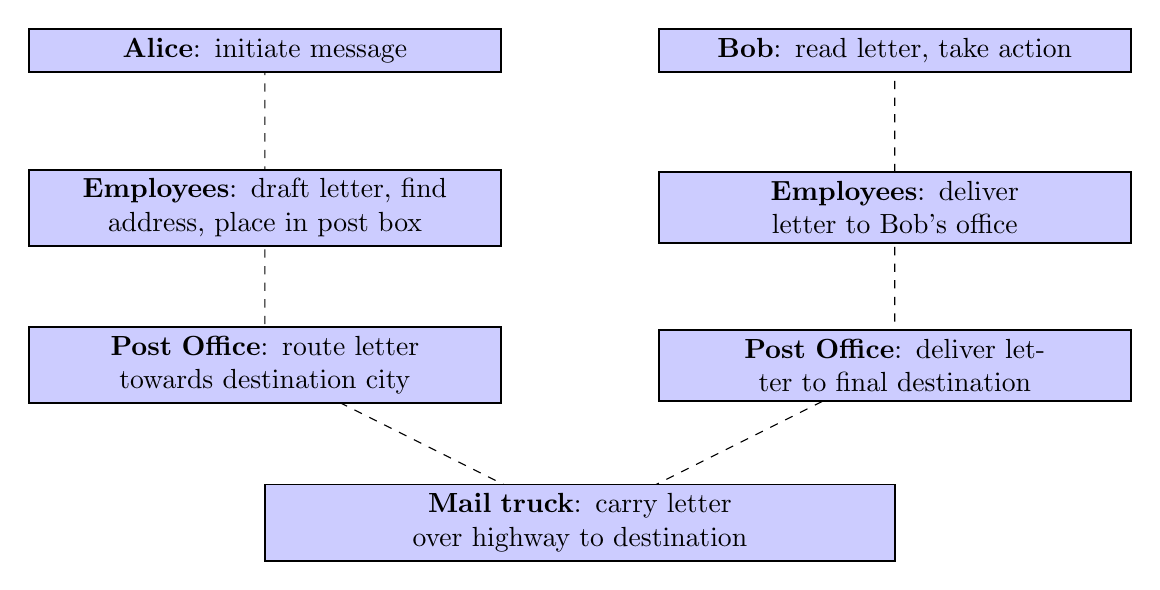
\begin{tikzpicture}[layer/.style={fill=blue!20,minimum width=6cm,align=center,text width=5.5cm,draw=black,solid,line width=.25mm}]
        \draw[dashed,-latex] (-4, 4) node[layer] {\textbf{Alice}: initiate message} --
        (-4, 2) node[layer] {\textbf{Employees}: draft letter, find address, place in post box} --
        (-4, 0) node[layer] {\textbf{Post Office}: route letter towards destination city} --
        (0, -2) node[layer,minimum width=8cm,text width=7.5cm] {\textbf{Mail truck}: carry letter over highway to destination} --
        (4, 0)  node[layer] {\textbf{Post Office}: deliver letter to final destination} --
        (4, 2)  node[layer] {\textbf{Employees}: deliver letter to Bob's office} --
        (4, 4)  node[layer] {\textbf{Bob}: read letter, take action};
    \end{tikzpicture}
    \caption{Layers of the postal system.}
    \label{fig:layer_mail}
\end{figure}

These layers all have counterparts in the Internet. At the top, we have the \emph{application layer}: programs which rely on the Internet and know how to initiate messages, much like Alice and Bob. The application layer relies on the \emph{transport layer} to determine an address where the messages should go, just as Alice relied on Jane to find Bob's mailing address. The transport layer relies on the \emph{Internet layer} to use the address to send the message to the right location, just as the Post Office routed Alice's letter to Bob's city. Finally, the transport layer relies on the \emph{link layer} to physically transmit data over wires or wireless protocols, just as the Post Office relies on mail trucks to move envelopes.

This set of four layers is commonly known as TCP/IP, named for the Transmission Control Protocol (TCP) which commonly runs the transport layer, and the Internet Protocol (IP) which commonly runs the Internet layer. The following sections contain more details on each of the layers. You should always keep in mind that these layers work together just like the layers of the postal system work together.

\subsection{Application Layer}

The application layer is the highest layer of TCP/IP. It consists of various protocols that specify how to send different types of data over the Internet. You might have heard of one of these protocols, HTTP. HTTP stands for HyperText Transfer Protocol. It comes at the beginning of a web address. When you type \texttt{http://www.google.com}, you're telling your computer to use HTTP to access \texttt{www.google.com}.

There are many other protocols in the application layer. HTTPS is a secure version of HTTP, which we'll discuss in Section \ref{sec:network:security}. Another popular protocol is SSH, or Secure Shell, which programmers use to access a Linux terminal on another Internet-connected machine. The file transfer protocol, or FTP, is used for exchanging files between different computers. A variety of protocols, such as POP3, IMAP, and SMTP, are used for exchanging emails.

When the application layer receives data from the transport layer, it needs to know which protocol it was sent over. In order to sort out all the different data, the application layer uses \emph{ports}. All Internet communications happen over some numbered port. For example, HTTP uses port 80. When you load \texttt{http://www.google.com}, your computer sends the request to Google over port 80. Google sends its home page back over port 80. Table \ref{tab:common_ports} lists the most commonly used protocols and the ports they use.

\begin{table}
    \centering
    \begin{tabular}{lll}
        Protocol & Port & Usage \\
        \hline
        HTTP & 80 & Web traffic \\
        HTTPS & 443 & Secure web traffic \\
        FTP & 21 & File transfer \\
        SSH & 22 & Remote shell access \\
        IMAP & 993 & Receiving email \\
        SMTP & 587 & Sending email
    \end{tabular}
    \caption{Commonly used Internet protocols.}
    \label{tab:common_ports}
\end{table}

If you write a program that uses the Internet, you will interact primarily with the application layer. A very common example is writing a program which runs on a web server. A web server is a computer which is connected to the Internet, and runs a program that constantly listens for incoming communications on ports 80 and 443 -- the ports used for the World Wide Web. When it receives a request, it will run a program and send the output of that program back to the requester. Every website is hosted by a web server, which knows how to send the data of the website to anyone who requests it.

A simple and famous example is \texttt{isitfriday.net}. This website is hosted by a server which listens for requests. When it gets a request for \texttt{isitfriday.net}, it will run a program which checks if it is Friday (you'll learn how to use ``if'' logic in programs in the next chapter). If it is Friday, it sends back a website that says ``Yes.'' Otherwise, it sends back a website that says ``Not yet.''

\subsection{Transport Layer}

When the application layer is ready to transmit a message, it will pass it down to the transport layer. By far the most common transport layer protocol is TCP, for Transmission Control Protocol. We will focus on TCP in this section. Another common protocol in the transport layer is TLS, for Transport Layer Security, which runs alongside TCP. We will discuss TLS more in Section \ref{sec:network:security}.

When TCP receives a request to transfer a message to a destination, it will first complete a ``handshake'' with that destination. The goal of the handshake is to establish that both parties are connected to the Internet and ready and willing to communicate with one another. TCP uses a three-way handshake: first the sender sends a signal to the receiver. The receiver replies with an acknowledgement of the signal, and a signal of its own. Finally, the sender acknowledges the signal from the receiver. At this point TCP can begin transmitting data.

When TCP receives a message for transfer, it will prepare to send it piece by piece over the network. The individual pieces are called \emph{packets}. These packets are relatively small, about a kilobyte. For reference, an average-sized image would typically be broken into a few thousand packets before being transferred. 

The reason for this is that a major role of TCP is to guarantee reliability. The application layer assumes that its message will be sent in full and without errors, while the Internet layer does not guarantee accurate or successful transmission, so it is the job of the transport layer to ensure robust communication. By breaking a message into packets, TCP helps to reduce the chance that any individual packet fails to transmit. In addition, if a packet does fail to transmit, it doesn't take too much time to recover, since TCP can re-send the relatively small packet.

\subsection{Internet Layer}

Perhaps the most interesting layer of the TCP/IP stack is the Internet layer, which almost always consists of the Internet Protocol (IP). This layer corresponds to the Post Office in our analogy: it is responsible for routing data where it needs to go. Just as the Post Office uses mailing addresses to specify locations, the Internet layer uses IP addresses to specify computers on the network.

An IP address is a sequence of 32 bits, grouped into blocks of 8. When they are written out, the groups of 8 bits are converted to decimal numbers between 0 and 255. The groups are separated by dots, so sometimes an IP address is referred to as a ``dotted quad.'' For example, the IP address \texttt{172.217.15.78} points to the server which hosts \texttt{www.google.com}. These addresses are stored in a sort of phone book called the Domain Name System, or DNS. When you type a website into your browser, it will first look up its IP address in the Domain Name System, and then request that IP address over the network.

When the Internet layer receives a packet from the transport layer for transmission, it will look at the IP address of the destination. It knows how to find a server which is closer to that destination. For example, if a server in New York City sees a packet destined for an IP address in Washington, DC., it might decide to forward that packet to a server in Philadelphia, PA.

You can view this process yourself using a Unix utility called \texttt{traceroute}. Open a terminal and type \texttt{traceroute} followed by any website. You'll see how the Internet Protocol routes your packets through different servers in order to reach their destination. For example, below is the route from a personal computer to \texttt{youtube.com}. The address in the last line, \texttt{172.217.12.238}, specifies the location of one of YouTube's servers.

\label{code:traceroute}
\begin{monospace}
# traceroute youtube.com
    1  192.168.1.1 (192.168.1.1)  0.448 ms  0.958 ms  0.966 ms
    2  * * *
    3  ae1312-21.ARTNVAFC-MSE01-AA-IE1.verizon-gni.net (100.41.21.152)  7.779 ms  7.766 ms  7.628 ms
    4  0.ae10.GW13.IAD8.ALTER.NET (140.222.225.219)  9.139 ms  9.117 ms  9.082 ms
    5  72.14.218.232 (72.14.218.232)  8.507 ms  7.277 ms  4.378 ms
    6  * * *
    7  216.239.54.106 (216.239.54.106)  4.779 ms 108.170.232.0 (108.170.232.0)  12.022 ms 108.170.246.33 (108.170.246.33)  16.086 ms
    8  108.170.246.67 (108.170.246.67)  12.976 ms 108.170.232.19 (108.170.232.19)  12.769 ms 108.170.246.66 (108.170.246.66)  10.935 ms
    9  iad30s15-in-f14.1e100.net (172.217.12.238)  10.570 ms 216.239.47.127 (216.239.47.127)  16.793 ms iad30s15-in-f14.1e100.net (172.217.12.238)  10.485 ms
\end{monospace}

The IP addresses we've described all correspond to version 4 of the Internet Protocol, or IPv4. There are about four billion unique IPv4 addresses, which seemed like plenty at the time of its creation. However, the growth of the Internet and the proliferation of mobile devices has led to the exhaustion of almost all IPv4 addresses. In order to ensure that the Internet can continue to grow, a transition to IPv6, which provides for many more addresses, is slowly taking place.

\subsection{Link Layer}

Finally, we come to the actual nuts and bolts of the Internet: how are individual pieces of data sent across the network? This part of networking is handled by the link layer.

There are two main link layer technologies you will encounter. The first is Ethernet, which is used for wired Internet connections. An Ethernet cable, also known as an RJ-45 cable, is shown in Figure \ref{fig:ethernet}. Each end of the cable has an 8-pin connector. Inside the cable, a twisted pair of wires can carry signals in both directions without having them collide with each other.

\begin{figure}
    \centering
    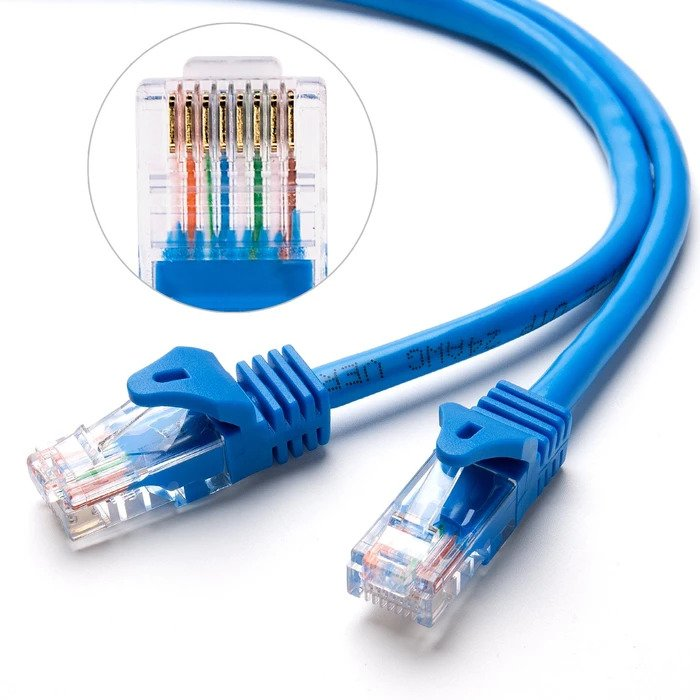
\includegraphics[width=.6\linewidth]{images/ethernet.jpg}
    \caption{An Ethernet cable used to network computers together.}
    \label{fig:ethernet}
\end{figure}

The other primary link layer technology is 802.11, more commonly known as Wi-Fi. With a wired network, signals can be sorted into separate wires so they don't overlap, but over a wireless network signals are broadcast and have the potential to interfere with one another. In order to prevent this, Wi-Fi is designed to allow devices to operate at slightly different frequencies which are arranged into channels.

There are two major variants of Wi-Fi: 2.4 gigahertz (GHz) and 5 GHz. These are two different frequency bands. Within each of them there are multiple channels. At 2.4 GHz, which was the first frequency available for Wi-Fi, there are 11 channels. However, the channels overlap with one another, so it is best for devices to use channels 1, 6, and 11, reducing the efffective number of channels down to 3. The newer 5 GHz protocol alleviates this problem by making hundreds of channels available. Most new devices can operate at either 2.4 GHz or 5 GHz, but some older devices only support 2.4 GHz.

The details of link layer technologies are complex, but luckily you rarely have to deal with them directly. In most cases, Ethernet or Wi-Fi have been engineered to the point where little effort is required to make them work properly, and you can focus on other layers of the network while trusting that signals are being carried appropriately by the link layer.

\section{Local Area Networks}

The network used to connect computers within a single home, business, or organization is called a local area network, or a LAN. Even though most LANs are connected to the outside Internet, they can also be used to allow devices on the same network to connect with each other without going through the Internet. In this section, we will review some concepts of local area networking and discuss using switches to manage network traffic.

\subsection{Network Topology}

When building a LAN, a network engineer has to connect computers either via Ethernet cables or wireless connections. For simplicity, we will focus on wired connections in this section.

In order to allow for a group of computers to communicate with each other, each computer must be able to reach any other computer via some number of hops in the network. The \emph{topology} of the network is the layout of the connections in the network, and this sets how a pair of computers communicates. 

One simple way to allow computers to communicate would be to connect all the computers in a line. Then each computer can communicate with the computers directly adjacent to it. This is called a linear topology, also known as daisy-chaining. Figure \ref{fig:daisy_chain} shows a network with linear topology.

\begin{figure}
    \centering
    \begin{tikzpicture}
        \node at (0,0) (a) {
\includegraphics[width=1cm]{images/computer.png}};
        \node at (3,0) (b) {
\includegraphics[width=1cm]{images/computer.png}};
        \node at (6,0) (c) {
\includegraphics[width=1cm]{images/computer.png}};
        \node at (9,0) (d) {
\includegraphics[width=1cm]{images/computer.png}};
        \draw[dashed,very thick] (a) -- (b) (b) -- (c) (c) -- (d);
    \end{tikzpicture}
    \caption{A network with linear topology.}
    \label{fig:daisy_chain}
\end{figure}

With a linear topology, if a computer wants to send a message to a computer which is not its neighbor, the intermediate computers have to carry the message along. In order to facilitate this, the destination address is included along with a packet. If a computer receives a packet and sees that the destination address is not its own, it will forward the packet along in the direction of the destination address.

One limitation of a linear topology is the difficulty of adding new devices to the network. Every time a new computer is being set up, it would have to be inserted somewhere in the line, causing temporary disruptions in the network. A possible alternative is a bus topology, in which all computers are connected to a central bus line. This layout is shown in Figure \ref{fig:bus}.

\begin{figure}
    \centering
    \begin{tikzpicture}
        \node at (0,0) (a) {
\includegraphics[width=1cm]{images/computer.png}};
        \node at (3,0) (b) {
\includegraphics[width=1cm]{images/computer.png}};
        \node at (6,0) (c) {
\includegraphics[width=1cm]{images/computer.png}};
        \node at (9,0) (d) {
\includegraphics[width=1cm]{images/computer.png}};
        \draw[dashed,very thick] (-1,-1) -- (10,-1);
        \draw[dashed,very thick] (a) -- (0,-1) (b) -- (3,-1) (c) -- (6,-1) (d) -- (9,-1);
    \end{tikzpicture}
    \caption{A network with bus topology.}
    \label{fig:bus}
\end{figure}

With a bus topology, a device can be added to the network simply by linking it to the bus line. When a computer wants to send a message on the network, it specifies the destination address and sends the message to the bus. All other computers receive the message, since they are also on the bus. The computer for which the message was intended can then read the message.

A clear problem with the bus and linear topologies is that several computers on the network are involved whenever two computers have to communicate. In the bus topology in particular, every message is broadcast, so there can be competition for network resources when multiple devices try to send messages at once.

In order to alleviate these difficulties, a network can be arranged in a star topology. In a star topology, shown in Figure \ref{fig:star} all computers are connected to one central device. When a computer wants to send a message, it will send it to the central device, which then forwards it on to the destination address. This way every communication happens with no more than two hops across the network, and only the central device is involved in facilitating communications.

\begin{figure}
    \begin{subfigure}{0.45\linewidth}
        \centering
        \begin{tikzpicture}
            \node at (0,0) (a) {
\includegraphics[width=1cm]{images/computer.png}};
            \node at (90:2) (b) {
\includegraphics[width=1cm]{images/computer.png}};
            \node at (-30:2) (c) {
\includegraphics[width=1cm]{images/computer.png}};
            \node at (-150:2) (d) {
\includegraphics[width=1cm]{images/computer.png}};
            \draw[dashed,very thick] (a) -- (b) (a) -- (c) (a) -- (d);
        \end{tikzpicture}
        \caption{A network with star topology.}
        \label{fig:star}
    \end{subfigure}%
    \hspace{.1\linewidth}%
    \begin{subfigure}{0.45\linewidth}
        \centering
        \begin{tikzpicture}
            \node at (0,0) (a) {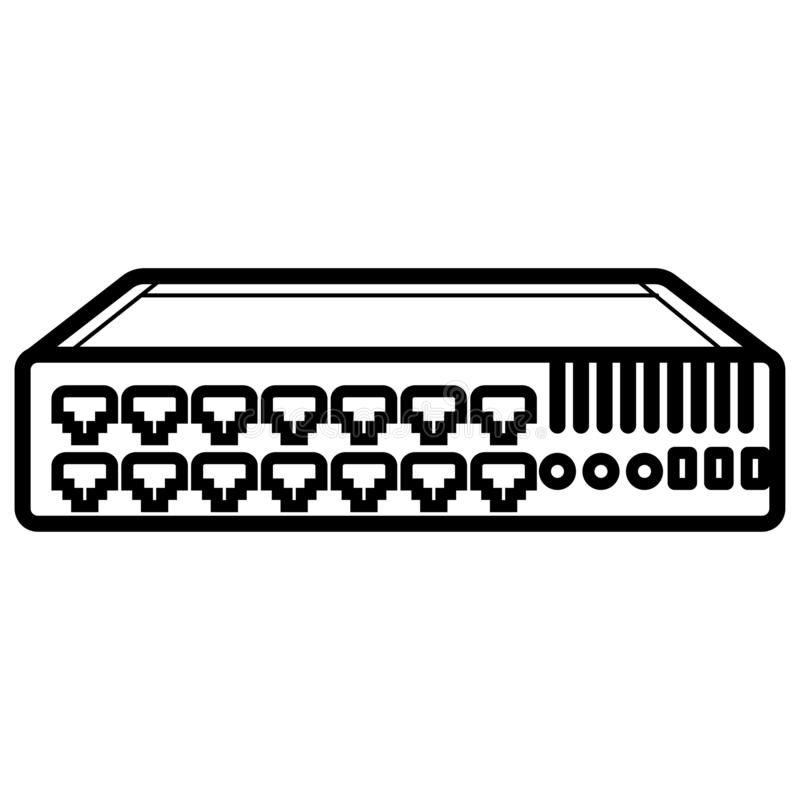
\includegraphics[width=1cm]{images/switch.jpg}};
            \node at (90:2) (b) {
\includegraphics[width=1cm]{images/computer.png}};
            \node at (-30:2) (c) {
\includegraphics[width=1cm]{images/computer.png}};
            \node at (-150:2) (d) {
\includegraphics[width=1cm]{images/computer.png}};
            \draw[dashed,very thick] (a) -- (b) (a) -- (c) (a) -- (d);
        \end{tikzpicture}
        \caption{A switched network.}
        \label{fig:switched}
    \end{subfigure}
    \caption{}
\end{figure}

In a star topology, the central device places an important and unique role. For this reason, it is very often replaced with a specialized network device called a switch. We will discuss switches in the following section.

\subsection{Switches}

A \emph{switch} is a device dedicated to moving packets through a network. It is designed to play the role of the central device in the star topology in Figure \ref{fig:star}. A typical switch may have dozens of Ethernet ports used to connect devices to it. The switch can receive packets from devices through these ports, and knows how to read the destination address of each packet. It forwards every packet along the cable pointing to the destination address, and nowhere else. This way, an Ethernet cable connected to a device is only every carrying packets sent from that device or intended for that device. A switched network is depicted in Figure \ref{fig:switched}.

It is useful to think about a switch in terms of the network layers we covered in Section \ref{sec:network:layers}. A switch is typically an Internet layer device. The Internet layer runs on top of the link layer, and so switches have link layer technology as well: these are the Ethernet ports and cables which allow devices to connect. Once a packet arrives at the switch, it uses the IP protocol in order to forward that packet to the appropriate device on the network. The flow of data from device to device follows the pattern in Figure \ref{fig:switch_layers}.

\begin{figure}
    \centering
    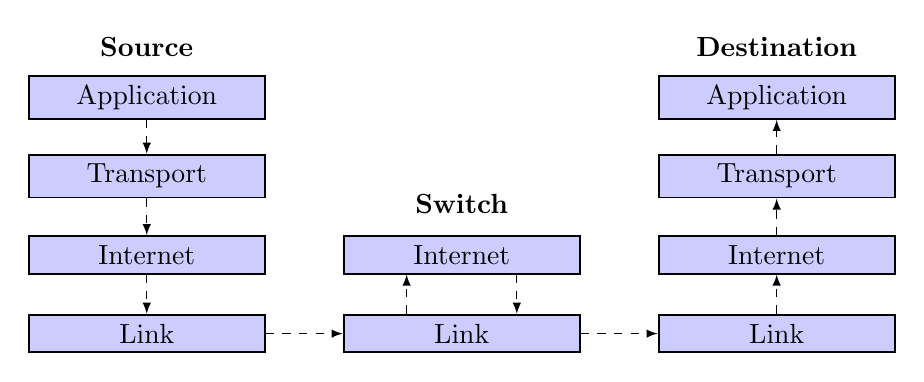
\begin{tikzpicture}[layer/.style={fill=blue!20,minimum width=3cm,align=center,text width=2.5cm,draw=black,solid,line width=.25mm},yscale=0.5]
        \node[above] at (-4, 4.8) {\textbf{Source}};
        \node[layer] at (-4, 4) (a1) {Application};
        \node[layer] at (-4, 2) (a2) {Transport};
        \node[layer] at (-4, 0) (a3) {Internet};
        \node[layer] at (-4, -2) (a4) {Link};

        \node[above] at (0, 0.8) {\textbf{Switch}};
        \node[layer] at (0, 0) (b1) {Internet};
        \node[layer] at (0, -2) (b2) {Link};

        \node[above] at (4, 4.8) {\textbf{Destination}};
        \node[layer] at (4, 4) (c1) {Application};
        \node[layer] at (4, 2) (c2) {Transport};
        \node[layer] at (4, 0) (c3) {Internet};
        \node[layer] at (4, -2) (c4) {Link};

        \draw[dashed,-latex] (a1) -- (a2);
        \draw[dashed,-latex] (a2) -- (a3);
        \draw[dashed,-latex] (a3) -- (a4);
        \draw[dashed,-latex] (a4) -- (b2);
        \draw[dashed,-latex,transform canvas={xshift=-.7cm}] (b2) -- (b1);
        \draw[dashed,-latex,transform canvas={xshift=.7cm}] (b1) -- (b2);
        \draw[dashed,-latex] (b2) -- (c4);
        \draw[dashed,-latex] (c4) -- (c3);
        \draw[dashed,-latex] (c3) -- (c2);
        \draw[dashed,-latex] (c2) -- (c1);
    \end{tikzpicture}
    \caption{The flow of data through network layers in a switched network.}
    \label{fig:switch_layers}
\end{figure}

Imagine a LAN with 50 devices connected to a switch. There are over a thousand different pairs of devices which may need to communicate with another, and the switch enables them to all communicate as if they had a dedicated cable between them, while actually using only 50 cables. This is the essential feature of any network: with relatively few physical connections, they enable an enormous number of potential communication channels. The Internet at large is designed in roughly the same way. We will discuss the details of the organization of the Internet, or more generally any wide area network, in the following section.

\section{Wide Area Networks}

Almost every LAN needs a way of communicating with the outside world. A network at a larger scale than a LAN is called a wide area network, or WAN. By far the most familiar example of a WAN is the Internet, but a WAN need not be this large. For example, a campus or metropolitan area may have its network organized as a WAN.

The link layer technology which carries signals over a WAN is similar to that of a LAN. A WAN typically needs higher capacity Ethernet cables, but the general principles are the same. The primary difference between a LAN and a WAN comes in at the Internet layer, where the IP protocol distinguishes between public and private networks. In this section we will discuss this difference, and the systems and protocols used to connect public networks together.

\subsection{Gateways and Routing}

If you have used a home network, you may be more familiar with routers than switches. This is because a switch is designed to connect all the devices into an area into a local network, but typically we also want to connect a local network to the outside Internet. This is the role of a router. Routers are responsible for connecting different networks together into a larger network.

In a typical setup, several devices on a local network will be connected to a router. The router assigns private IP addresses to each of these devices. Private IP addresses belong to one of three special blocks reserved for this purpose. The most common block is 192.168.*.*, any address ranging from 192.168.0.0 to 192.168.255.255. There are about 65,000 such addresses. A block like this can be written as 192.168.0.0/16, meaning the first 16 bits are fixed and the rest can change. The other private IP address ranges are 172.16.0.0/12, with about 1 million addresses, and 10.0.0.0/8, with about 16 million addresses.

When a device (such as a switch) within the LAN receives a packet, it will look at the destination IP address. If it knows where to route the packet -- that is, if the packet is destined for another device on the local network -- then it will forward the packet appropriately. If it does not know where to route the packet, then it will forward it on to the device designated as the \emph{default gateway} for the network. The default gateway is typically the router.

When the router receives a packet with a destination address outside the local network, it knows how to forward it appropriately. First, it will change the source address of the packet. The packet originated from a device on the private network, so its source address is a private address, such as 192.168.1.4. The router will replace this source address with its own address on the WAN. This will be a public IP address, such as 172.217.15.100. It then sends the packet out to the public Internet and awaits a reply. When it receives a reply, it will forward the packet on to the correct device on the network. This process is depicted in Figure \ref{fig:gateway}.

\begin{figure}
    \centering
    \begin{tikzpicture}
        \useasboundingbox (-8,-1.5) rectangle (5,2.5);
        \begin{scope}[transform canvas={scale=.8}]
        \node[label={[align=center]90:Private: 192.168.1.1\\Public: 172.217.15.100}] at (0,0) (a) {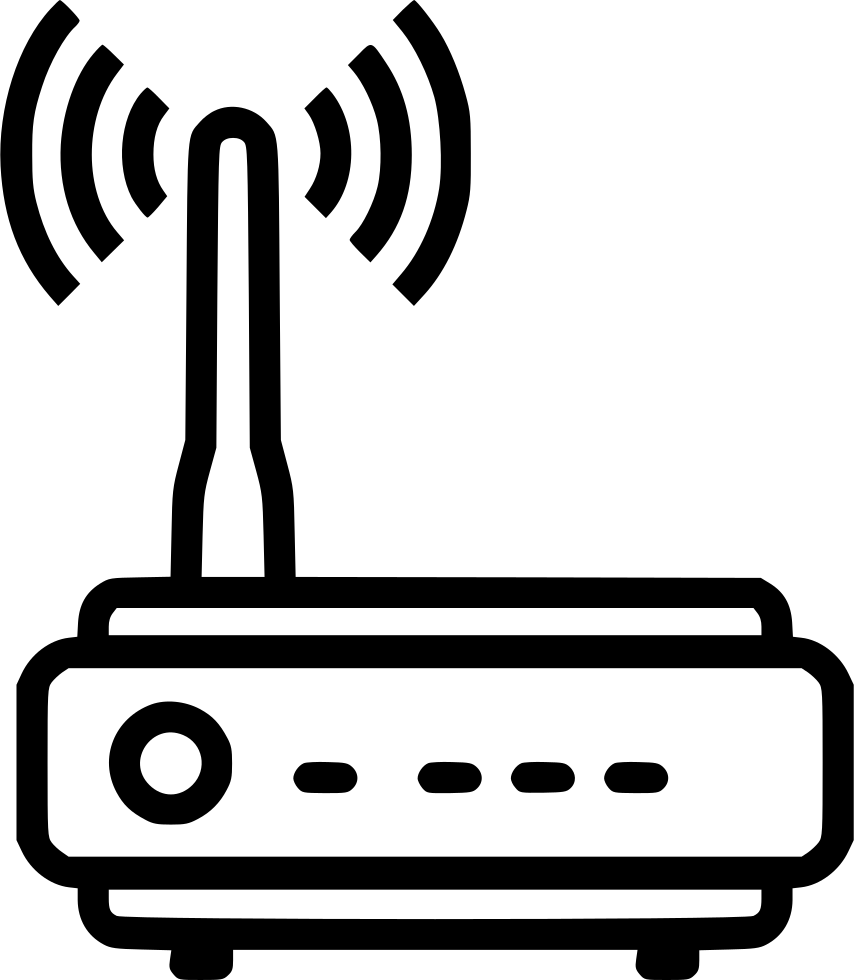
\includegraphics[width=1cm]{images/router.png}};
        \node[label={180:192.168.1.2}] at (-5,2) (b) {
\includegraphics[width=1cm]{images/computer.png}};
        \node[label=180:{192.168.1.3}] at (-6,1) (c) {
\includegraphics[width=1cm]{images/computer.png}};
        \node[label=180:{192.168.1.4}] at (-7,0) (d) {
\includegraphics[width=1cm]{images/computer.png}};
        \draw[dashed,very thick] (b) -- (a) (c) -- (a) (d) -- (a);
        \node[draw,thick,right,align=left] at (-6,-0.7) (packet) {\scriptsize Source: 192.168.1.4\\\scriptsize Destination: 208.80.153.224};
        \draw[thick,->] (packet) -- (-1.5,-0.7);
        \node[draw,thick,right,align=left] at (2,-0.7) (packet2) {\scriptsize Source: 172.217.15.100\\\scriptsize Destination: 208.80.153.224};
        \draw[thick,->] (1,-0.7) -- (packet2);
        \draw[dashed,very thick] (a) -- ++(5,0) node[above left] (cloud) {
\includegraphics[width=2cm]{images/cloud.png}};
        \node at (cloud) {Internet};
        \end{scope}
    \end{tikzpicture}
    \caption{The default gateway forwards packets from a LAN to a WAN.}
    \label{fig:gateway}
\end{figure}

\subsection{Autonomous Systems}

Once a packet is routed to a wide area network, such as the Internet, it needs to be sent to the network which contains the destination address. Typically, the first destination for a packet is a router belonging to an Internet Service Provider (ISP). For example, in the \texttt{traceroute} trace on page \pageref{code:traceroute}, the packet ends up at a router owned by Verizon, a popular ISP. This router belongs to an \emph{autonomous system} (AS) operated by Verizon. An autonomous system is simply a connection of routers on the Internet which are under some common administrative control, such as by an ISP.

Autonomous systems are managed globally using autonomous system numbers, or ASNs, which are similar to IP addresses. These numbers are allocated by the Internet Assigned Numbers Authority (IANA) to Regional Internet Registries (RIRs), which then assign the numbers to autonomous systems.

The routers in an autonomous system can forward packets to destinations within the same AS, but if a packet is destined for a network on another AS, it needs to be routed appropriately. This requires different ASs to communicate with one another. This can happen via \emph{peering}, in which two ASs mutually agree to carry traffic to one another free of charge, or via \emph{transit}, in which an AS charges a fee to carry traffic from other ASs.

When two ASs need to communicate with one another, they use the Border Gateway Protocol (BGP). This is the core routing protocol of the Internet, and is responsible for making decisions on how to get packets to a destination in the quickest way possible. 

\section{Network Security}\label{sec:network:security}

One of the most important issues with computer networks is security. The Internet is frequently used for transmitting confidential messages, facilitating financial transactions, and other applications where security is paramount. For this reason,there are protocols dedicated to ensuring that the Internet can be secure. The most common such protocol is Transport Layer Security (TLS), which is a successor to an older protocol called Secure Sockets Layer (SSL). TLS is implemented at the transport layer of a network. Web traffic which uses TLS/SSL security is sent using the HTTPS protocol at the application layer, rather than the unsecured HTTP protocol.

Another common network security application is a Virtual Private Network, or VPN. A VPN allows computers connected to different LANs to communicate over the Internet as if they belonged to the same LAN. This is often used by companies to allow employees to access private resources even when they are away from the office. Security is very important for a VPN, and it can be provided using TLS or other protocols.

The details of TLS are complicated, and we will not get into them here. Instead, we will cover what exactly security means in a network setting, and look at three goals of any secure network: privacy, authenticity, and reliability. Achieving these goals requires using tools from cryptography, which you may learn about in a future course.

\subsection{Privacy}

When two parties want to securely transmit a message, one of their most straightforward goals is privacy. The two parties do not want a third party to be able to lisen in on their communication.

Following a standard convention in cryptography, we will denote the two parties by Alice and Bob, and the adversarial third party by Carol. Alice is sending a message to Bob, and Carol wants to listen in. Since network signals travel over cables, Carol could listen in to the signal by physically tapping into a wire. Even more easily, on a wireless network, all signals are broadcast over the air and can be received by anyone who wants to listen.

In order to protect their messages from being read by Carol, Alice and Bob use an encryption algorithm. Alice and Bob have some shared key, and when Alice wants to send a message, she first uses her key to turn the plain text of the message into a cipher text. If the algorithm is secure, then the cipher text cannot be converted back to the plain text without knowledge of the key. This way, if Carol manages to read the message, she will only see nonsensical cipher text. Only Bob, who has the key, can produce the plain text.

A key issue here is how Alice and Bob come to have the same key. If Alice tells Bob her key over the network, then Carol could retrieve the key and use it to decrypt all future messages. This is a fundamental problem in cryptography called the key-sharing problem. It is solved using a technique called public key cryptography. In TLS, public key cryptography is implemented using either the RSA algorithm, or a more sophisticated method called elliptic curve cryptography (ECC). These algorithms allow Alice and Bob to generate shared keys which Carol cannot intercept.

\subsection{Authenticity}

Even if Carol cannot read messages sent between Alice and Bob, she can still do damage. One potential attack would be for Carol to impersonate Alice, by sending a message to Bob which says it comes from Alice. This is why TLS must also protect the authenticity of messages: if a message says it comes from Alice, Bob needs some way of verifying that this is actually the case.

The public key cryptography algorithms used for ensuring privacy can also provide authenticity. In these algorithms, every party on the network has a private key which is never shared with anyone. This private key is important for generating the shared keys used for encrypting messages. It can also be used to generate a ``digital signature,'' which could only be produced by someone in possession of the private key. As long as the private key has never been shared, a digital signature can provide a guarantee of authenticity.

\subsection{Integrity}

Finally, even if Carol cannot read messages or impersonate Alice or Bob, she could try to modify one of their messages. This is called a man-in-the-middle (MITM) attack, where Carol intercepts Alice's communications, edits them, and then forwards them to Bob with Alice's signature intact.

To protect against this, TLS uses a message authentication code (MAC) which is sent along with any message. This is a short code sent with the message, which depends on the shared key and on the message. If the algorithms are secure, then it should be nearly impossible to generate a MAC without knowledge of both the shared key and the message. When Bob receives the message along with the MAC, he verifies that the MAC is correct. If it is not, then he knows the message has been altered in transit and discards it.

\subsection{Security versus Trust}

An enormous amount of expertise, testing, and iteration has gone into making TLS secure. However, it is still relatively common to hear about security problems on the Internet. Where do these problems come from?

In this context, it is important to recognize a key difference between security and trust. Network security provided by TLS achieves the three goals outlined above: privacy, authenticity, and integrity. When Alice communicates with Bob, she can be sure that only Bob can read her messages, that messages she receives from Bob really come from Bob, and that the messages have not been altered in transit. However, \emph{TLS does not guarantee that Alice can trust Bob}.

There are many ways in which Bob could be unreliable. For example, Bob could be attempting to execute a phishing attack by impersonating someone else. TLS guarantees that Bob cannot truly impersonate \texttt{facebook.com}, but he could own \texttt{fcebook.com} and, using TLS security, provide a website that looks just like \texttt{facebook.com} and asks for your login credentials. If you provide them to \texttt{fcebook.com}, then Bob could read your password and log into your actual Facebook account.

Even if Bob is not malicious, he could be irresponsible. For example, if Bob runs an online vendor which collects credit card information to make payments, it is crucial that Bob takes appropriate security measures on his local network to protect that credit card information from becoming known to an attacker. TLS does not guarantee that Bob has taken the necessary precautions. Many of the most substantial security problems arise on the Internet when many customers have trusted a vendor like Bob with their personal details like credit card numbers, and Bob suffers a data breach, putting this data into the wrong hands.

Network security is an evolving field as companies and governments work to protect against these sorts of vulnerabilities. There are many opportunities for employment in this area, as organizations increasingly need to rely on dedicated security professionals in order to keep their data and their clients' data safe.